%%% Template originaly created by Karol Kozioł (mail@karol-koziol.net) and modified for ShareLaTeX use

\documentclass[a4paper,11pt]{article}

\usepackage[T1]{fontenc}
\usepackage[utf8]{inputenc}
\usepackage{graphicx}
\usepackage{xcolor}

\renewcommand\familydefault{\sfdefault}
\usepackage{tgheros}
\usepackage[defaultmono]{droidmono}

\usepackage{amsmath,amssymb,amsthm,textcomp}
\usepackage{enumerate}
\usepackage{multicol}
\usepackage{tikz}
\usetikzlibrary{arrows}

\usepackage{geometry}
\geometry{total={210mm,297mm},
left=25mm,right=25mm,%
bindingoffset=0mm, top=20mm,bottom=20mm}


\linespread{1.3}

\newcommand{\linia}{\rule{\linewidth}{0.5pt}}

% custom theorems if needed
\newtheoremstyle{mytheor}
    {1ex}{1ex}{\normalfont}{0pt}{\scshape}{.}{1ex}
    {{\thmname{#1 }}{\thmnumber{#2}}{\thmnote{ (#3)}}}

\theoremstyle{mytheor}
\newtheorem{defi}{Definition}

% my own titles
\makeatletter
\renewcommand{\maketitle}{
\begin{center}
\vspace{2ex}
{\huge \textsc{\@title}}
\vspace{1ex}
\\
\linia\\
\@author \hfill \@date
\vspace{4ex}
\end{center}
}
\makeatother
%%%

% custom footers and headers
\usepackage{fancyhdr}
\pagestyle{fancy}
\lhead{}
\chead{}
\rhead{}
\lfoot{Assignment \textnumero{} 2}
\cfoot{}
\rfoot{Page \thepage}
\renewcommand{\headrulewidth}{0pt}
\renewcommand{\footrulewidth}{0pt}
%

% code listing settings
\usepackage{listings}
\lstset{
    language=Python,
    basicstyle=\ttfamily\small,
    aboveskip={1.0\baselineskip},
    belowskip={1.0\baselineskip},
    columns=fixed,
    extendedchars=true,
    breaklines=true,
    tabsize=4,
    prebreak=\raisebox{0ex}[0ex][0ex]{\ensuremath{\hookleftarrow}},
    frame=lines,
    showtabs=false,
    showspaces=false,
    showstringspaces=false,
    keywordstyle=\color[rgb]{0.627,0.126,0.941},
    commentstyle=\color[rgb]{0.133,0.545,0.133},
    stringstyle=\color[rgb]{01,0,0},
    numbers=left,
    numberstyle=\small,
    stepnumber=1,
    numbersep=10pt,
    captionpos=t,
    escapeinside={\%*}{*)}
}

\tikzstyle{arn_n} = [circle, white, font=\bfseries, draw=black, fill=black, align=center, inner sep=0pt,text width=1.5em, text centered]% black node
\tikzstyle{arn_r} = [circle, red, draw=red, align=center, inner sep=0pt,text width=1.5em, text centered, very thick]% red node
\tikzstyle{arn_x} = [rectangle, draw=black, align=center, inner sep=0pt,minimum width=0.5em, minimum height=0.5em]% NIL 'node'

%%%----------%%%----------%%%----------%%%----------%%%

\begin{document}

\title{Theoretical Assignment \textnumero{} 2}

\author{Harsh Sinha(14265), Deepak Gangwar(14208)}

\date{09/03/2017}

\maketitle

\section*{Problem 1}

The pseudo code is as follows.

\begin{lstlisting}[label={list:first},caption=Pseudo code -- Search in an Infinite Array.]
BOOL infinite_search{
isfound = FALSE;
i = 1;
s = s;
while (isfound == 0)
{
	if (A[i] == s)
		isfound = TRUE;
	else if (A[i] < s)
		i = i * 2;
	else if (A[i] > s OR A[i] == empty)
		modif_bin_search (i);
}
return isfound;
}
\end{lstlisting}

\begin{lstlisting}[caption=modif\_bin\_search.]
void modif_bin_search (int i)
{
	L = i / 2;
	R = i;
	mid = (L + R) / 2
	while (mid != R)
	{
		if (A[mid] == s)
			return;
		else if (A[mid] < s)
			L = mid + 1;
		else if (A[mid] > s OR A[mid] == empty)
			R = mid -1;	
	}
}
\end{lstlisting}

\textbf{Proof of correctness}\\
TODO fill here.\\
\\

\textbf{Time Complexity}\\
The function modif\_bin\_search takes log(i) steps to give us a solution (Similar to a binary search). Now the original function in the worst case takes log(n) steps. Thus in the worst possible case our algorithm shall consume 2 * log (n). Hence, the order of the given algorithm is log (n).\\
This can also be proposed by saying that the number of elements that this algorithm skips keeps on doubling every loop and so the order should be log (n).\\
Notice that the base of log (n) is decided based on our choice of the multiplier in every step.
\section*{Problem 3}
\textbf{Part (a)} Deleting 55 \\
\textbf{Part (b)} Inserting 34 \\
%%%%%%%%%% Step 1 %%%%%%%%%%%%%
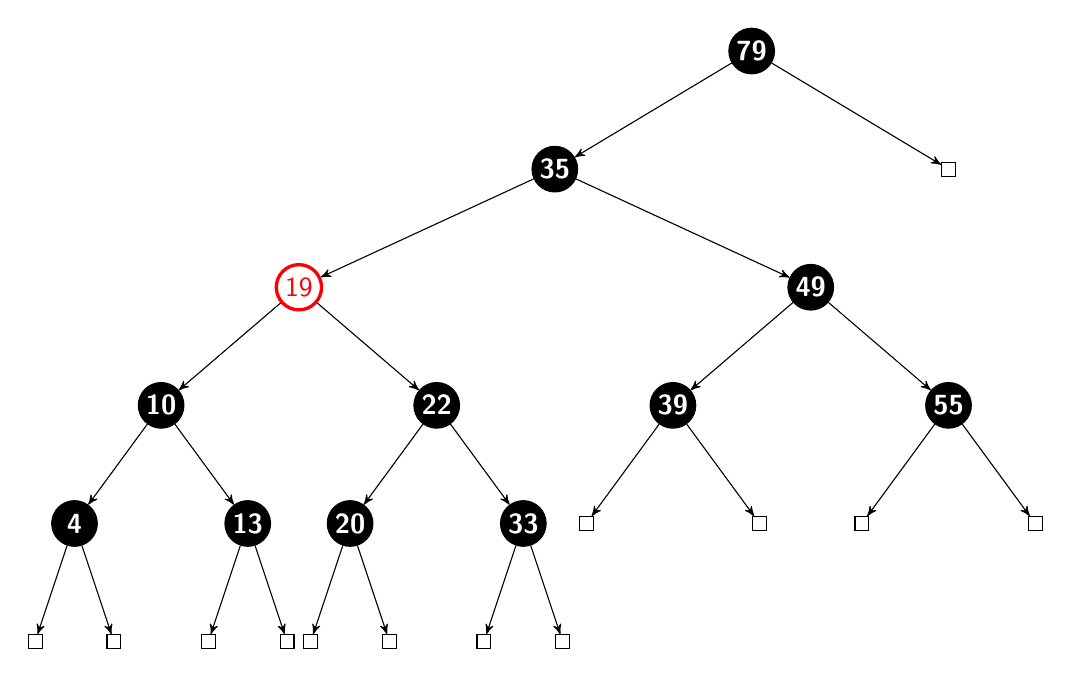
\begin{tikzpicture}[->,>=stealth',level/.style={sibling distance = 5cm/#1, level distance = 1.5cm},
level 2/.style={sibling distance = 6.5cm},
level 3/.style={sibling distance = 3.5cm},
level 4/.style={sibling distance = 2.2cm}
] 
\node [arn_n] {79}
    child{ node [arn_n] {35}
        child{ node [arn_r] {19} 
            child{ node [arn_n, name=leaf 5] {10}
            	child{ node [arn_n] {4}
					child{ node [arn_x] {}}
					child{ node [arn_x] {}}           		
            		}            	
				child{ node [arn_n] {13}
					child{ node [arn_x] {}}
					child{ node [arn_x] {}}
					}
            	}
            child{ node [arn_n] {22}
				child{ node [arn_n] {20}
					child{ node [arn_x] {}}
					child{ node [arn_x] {}}				
				}
				child{ node [arn_n] {33}
					child{ node [arn_x] {}}
					child{ node [arn_x] {}}		
					}
            	}
        	}
        child{ node [arn_n] {49}
            child{ node [arn_n] {39}
					child{ node [arn_x] {}}
					child{ node [arn_x] {}}
            }
            child{ node [arn_n] {55}
					child{ node [arn_x] {}}
					child{ node [arn_x] {}}            
            }
        }                            
    }
    child{ node [arn_x] {}
    }
; 
\end{tikzpicture}
%%%%%%%%%% Step 1 end %%%%%%%%%%%%%
\linebreak
%%%%%%%%%% Step 2 begin %%%%%%%%%%%%%
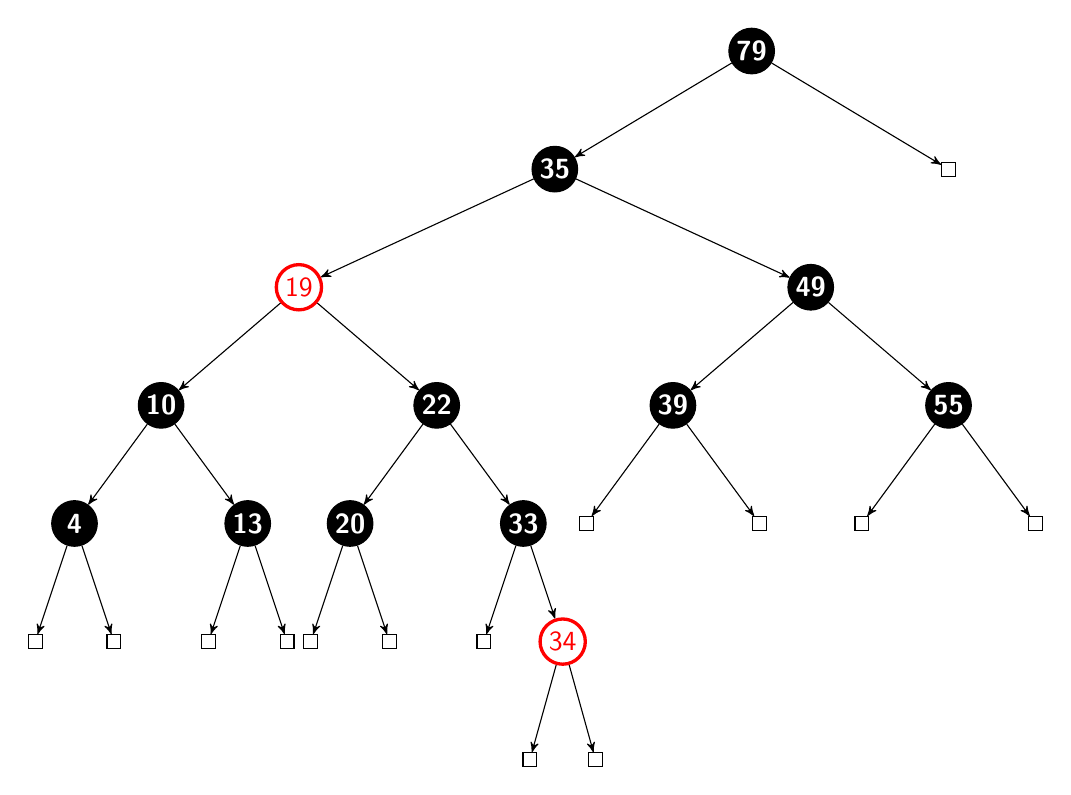
\begin{tikzpicture}[->,>=stealth',level/.style={sibling distance = 5cm/#1, level distance = 1.5cm},
level 2/.style={sibling distance = 6.5cm},
level 3/.style={sibling distance = 3.5cm},
level 4/.style={sibling distance = 2.2cm}
] 
\node [arn_n] {79}
    child{ node [arn_n] {35}
        child{ node [arn_r] {19} 
            child{ node [arn_n, name=leaf 5] {10}
            	child{ node [arn_n] {4}
					child{ node [arn_x] {}}
					child{ node [arn_x] {}}           		
            		}            	
				child{ node [arn_n] {13}
					child{ node [arn_x] {}}
					child{ node [arn_x] {}}
					}
            	}
            child{ node [arn_n] {22}
				child{ node [arn_n] {20}
					child{ node [arn_x] {}}
					child{ node [arn_x] {}}				
				}
				child{ node [arn_n] {33}
					child{ node [arn_x] {}}
					child{ node [arn_r] {34}
						child{ node [arn_x] {}}
						child{ node [arn_x] {}}						
						}		
					}
            	}
        	}
        child{ node [arn_n] {49}
            child{ node [arn_n] {39}
					child{ node [arn_x] {}}
					child{ node [arn_x] {}}
            }
            child{ node [arn_n] {55}
					child{ node [arn_x] {}}
					child{ node [arn_x] {}}            
            }
        }                            
    }
    child{ node [arn_x] {}
    }
; 
\end{tikzpicture}
%%%%%%%%%% Step 2 end %%%%%%%%%%%%%
\end{document}
